\RequirePackage{fixltx2e} %This package in CTeX is not compatible with revtex4-1
\documentclass[aps,pre,12pt,preprint,onecolumn,showpacs,showkeys]{revtex4-1}
\usepackage{ctex}
\usepackage{mathtools}
\usepackage{multirow}
\usepackage{setspace,dcolumn}
\usepackage{subfig}
\usepackage{hyperref}
\usepackage{graphicx,psfrag,epsfig}
\usepackage[font=small,format=plain,labelfont=bf,textfont=it,justification=centering,singlelinecheck=false]{caption}
\usepackage{amsmath,amsfonts,amssymb,amsthm,bm,upgreek}
\usepackage{geometry}
\usepackage[mathscr]{eucal}
\hypersetup{colorlinks=true}
\geometry{top=2.54cm,bottom=2.54cm,left=3cm,right=3cm}
\renewcommand\appendixname{附录}
\renewcommand\abstractname{}%摘要
\renewcommand\tablename{表}
\renewcommand\figurename{图}
\makeatletter
\def\@pacs@name{\songti\zihao{-4}{\bf PACS码:}}
\def\@keys@name{\songti\zihao{-4}{\bf 关键词:}}
\def\Dated@name{日期:}
\def\Received@name{\zihao{-5}{接收} }
\def\Revised@name{\zihao{-5}{修订} }
\def\Accepted@name{\zihao{-5}{采纳} }
\def\Published@name{\zihao{-5}{发表} }
\makeatother
\linespread{1.3}
\renewcommand{\labelenumi}{\alph{enumi}.}
\leftmargini=20mm
\def \d {\mathrm d}
\def \cs {\frac{\d \sigma}{\d \Omega}(\theta)}
\def \csref {\frac{\d \sigma}{\d \Omega}(\theta_0)}
\def \degree {^\circ}
\def \F {^{19}\mathrm{F}}

\begin{document}
\title{\bf\heiti\zihao{3}康普顿散射\vspace{15mm}}
\author{\fangsong\zihao{4}邵智轩\vspace{2mm}}
\affiliation{\songti\zihao{-4}学号:1400012141\vspace{2mm}}
\date{\today}
%\pacs{02.10.Yn, 33.15.Vb, 98.52.Cf, 78.47.dc}
\keywords{核磁共振,核磁矩,磁旋比,共振频率,Boltzman分布,拉莫进动,弛豫时间}
\email{shaozhixuansh@pku.edu.cn; (86)13381350619}

\begin{abstract}
\vspace{10mm}
\begin{spacing}{1.5}
\songti\zihao{-4}
本次实验的目的旨在掌握稳态核磁共振现象的原理和方法。实验用边限振荡器产生的射频连续波作用于磁场中的样品,利用共振时样品对射频场的吸收引起的震荡线圈$Q$值变化所导致的震荡信号变化进行检波来获得共振信号。本实验观察了水样品(掺有$\mathrm{FeCl_3}$)中质子的共振信号,并校准磁场;测量了聚四氟乙烯样品中$\F$核的$g$因子,并通过实验对横向弛豫时间$T_2$给出了估计

\end{spacing}
\end{abstract}
\maketitle
\songti\zihao{-4}

\section{引言}
1930年代,I.I.Rabi 利用原子束和不均匀磁场研究原子核磁矩时观察到核磁共振(NMR)现象。迄今为止,在核磁共振领域的研究发现和发明已五次获得诺贝尔奖。

核磁共振是基于原子尺度的量子磁物理性质。具有奇数质子或中子的核子,具有内在的核自旋,从而产生磁矩。在外加磁场下,空间取向量子化的磁矩能量是量子化的,造成能级的塞曼分裂。此时若在垂直于磁场方向施加一个频率合适的交变电磁场,将导致原子核在相邻的塞曼能级之间跃迁,这就是磁共振。

人们在发现核磁共振现象之后很快就产生了实际用途,化学家利用分子结构对氢原子周围磁场产生的影响,发展出了核磁共振谱,用于解析分子结构。另一方面,医学家们发现水分子中的氢原子可以产生核磁共振现象,利用这一现象可以获取人体内水分子分布的信息,从而精确绘制人体内部结构。在这一理论基础上,纽约州立大学石溪分校的物理学家保罗·劳特伯于1973年开发出了基于核磁共振现象的成像技术(MRI)。随着MRI技术日趋成熟,应用范围日益广泛,成为一项常规的医学检测手段。

\section{原理}
\subsection{原子核的磁矩}
角动量$\bm{P}$不为零的原子核具有平行(或反平行)的磁矩$\bm{\mu}$,而且有
\begin{equation}
\bm{\mu}=\gamma \bm{P}=g \cdot \frac{q}{2m_N} \bm{P}
\end{equation}
其中$\gamma$称为原子核的磁旋比,$g$为一个量纲为1的因子。按照经典理论,$g=1$,然而这与实验不符。实验测得质子的$g=5.59$,中子的$g=-3.82$。

对于质子,对应于玻尔磁子可以引入核磁子
$$\mu_N=\frac{e\hbar}{2 m_p}=5.0493\times10^{-27} \mathrm{J/T}$$
则质子的磁旋比
\begin{equation}
\frac{\bm{\mu}/\mu_N}{\bm{P}/\hbar}=\frac{\bm{\mu}}{\bm{P}}\frac{2m_p}{e}=g=\frac{\gamma}{\mu_N/\hbar}
\end{equation}
从而$g=\frac{\gamma}{\mu_N/\hbar}$,因此$g$和$\gamma$都可以表征原子核的磁旋比。
\subsection{磁能级与共振条件}
磁矩和外磁场的相互作用能也是不连续的,形成分立的能级
$$E=-\bm{\mu}\cdot \bm{B}=-\mu_z B=-m\gamma \hbar B, \ m=I,...,-I$$
两个相邻能级之间的能量差为
$$\Delta E=\gamma \hbar B$$
当垂直于恒定磁场$B$的平面上同时存在一个射频场,其频率$\nu$满足$h\nu=\Delta E$时,将发生磁偶极共振跃迁。即共振条件为
\begin{equation}
\omega = \gamma B \mbox{ 或 }\nu=\frac{\gamma}{2\pi}B
\end{equation}
通常把$\frac{\gamma}{2\pi}$称为原子核的回旋频率,单位为$\mathrm{MHz/T}$。若已知磁场$B$,测量共振频率可求出$\gamma/2\pi$的值;反之可通过已知回旋频率的原子核校准磁场。
\subsection{玻尔兹曼分布与能级的量子数差}\label{BM}
在热平衡时,上下能级粒子数遵从BM分布
\begin{equation}
\frac{N_{20}}{N_{10}}=\exp(-\Delta/kT)
\end{equation}
$N_{20}$、$N_{10}$分别是上、下能级的粒子数。一般情况下,$\Delta E \ll kT$,
$$\frac{N_{20}}{N_{10}}\approx1-\frac{\Delta E}{kT}=1-\frac{\gamma \hbar B}{kT}$$
由此可求出热平衡时下能级与上能级的粒子数之差
\begin{equation}
n_0=N_{10}-N_{20}\approx \frac{\gamma \hbar B}{2 k T} N 
\end{equation}
对于氢核,室温下磁场为$1\mathrm T$时,$n_0\approx 0.0000034 N$。就是这样微小的差数,提供了观察核磁共振的可能性。

\subsection{微观磁矩的拉莫进动}
自旋非零的粒子,在外磁场$\bm{B}$中受到一个力矩$\bm{L}=\bm{\mu}\times \bm{B}$,角动量$\bm{P}$的运动方程为
$$\frac{\d \bm{P}}{\d t}=\bm{L}=\bm{\mu}\times \bm{B}$$
考虑到$\bm{\mu}=\gamma \bm{P}$,有
\begin{equation}
\frac{\d \bm{\mu}}{\d t}=\gamma \bm{\mu} \times \bm{B}\label{moment_eq}
\end{equation}
上式即微观磁矩在外磁场中的运动方程。

若外加恒定磁场,方向沿$z$轴,则求解运动方程 (\ref{moment_eq}),可得磁矩$\bm{\mu}$绕静磁场进动,其在$x-y$平面上投影的大小为常量,进动角频率$\omega_0=|\gamma B_z|$,称为拉莫频率,它与$\bm{\mu}$和$\bm{B}$之间的夹角$\theta$无关。

\begin{figure}[h]
\centering
\includegraphics[width=100mm]{processing}
\caption{\label{fig:processing}%
旋转磁场$\bm{B}_1$的频率与进动频率相同时,磁矩$\bm{\mu}$在磁场$\bm{B}$中的能量增加(如(a))或减少(如(b))}
\end{figure}

如果我们在$x-y$平面上再加一个射频场$\bm{B}_1$,其角频率也为$\omega_0$。为了方便研究此时$\bm{\mu}$的运动,我们取以$\bm{B}_z$为轴,角速度为$\omega_0$的旋转坐标系。在该旋转坐标系中,磁矩$\bm{\mu}$保持不动,而新加的射频场$\bm {B}_1$以恒定场出现。因此$\bm{\mu}$在力矩$\bm{\mu}\times \bm{B}_1$的作用下将开始绕着$\bm{B}_1$进动。如图\ref{fig:processing}所示,$\bm{B}_1$对$\bm{\mu}$产生的力矩$\bm{\mu}\times \bm{B}_1$使$\bm{\mu}$与$\bm{B}_z$之间的的夹角$\theta$增加或减小,从而$\bm{\mu}$在外磁场$\bm{B}_z$中的能量
\begin{equation}
E=-\bm{\mu}\cdot \bm{B}_z=-\mu B_z \cos \theta
\end{equation}
也相应地增加或减小。这一能量变化可以借助于外电路加以探测。

\subsection{磁化强度矢量$M$的平衡值及不平衡趋向平衡的弛豫时间$T_1$和$T_2$}
单位体积中微观磁矩矢量的总和称为磁化强度矢量$\bm{M}=\sum_i\bm{\mu}_i$,它的运动方程与$\bm{\mu}$类似:
\begin{equation}
\frac{\d \bm{M}}{\d t}=\gamma \bm{M}\times \bm{B}_0
\end{equation}
$\bm{M}$也以圆频率$\omega_0 = \gamma B_0$绕外磁场$\bm{B}_0$进动。

在热平衡时,由\ref{BM}中结论,能量较低的磁矩取向的粒子总数$N_{10}$将多于能量较高的磁矩取向的粒子总数$N_{20}$;另外,由于拉莫进动的相位分布是随机的,单位体积的磁化强度矢量$\bm{M}$只有沿外磁场$z$方向的分量$M_0$,即$M_{x0}=M_{y0}=0$,$M_{z0}=M_0$。若在$x-y$平面上施加频率等于$\omega_0$的相干射频场,使$M_x$、$M_y$、$M_z$偏离热平衡值,这时存在磁化强度矢量$\bm{M}$趋于热平衡值的自发过程,称为弛豫。

表征$M_z$值恢复到热平衡值快慢的特征时间$T_1$称为纵向弛豫时间;表征$M_x$、$M_y$恢复到热平衡值快慢的特征时间$T_2$称为横向弛豫时间。$T_1$的大小取决于自旋系统和晶格的相互作用,自旋系统与晶格交换能量,使能级分布回归热平衡;$T_2$的大小不仅和自旋—晶格相互作用有关,还和自旋—自旋相互作用有关,它不改变能级分布与系统的总能量,但它使得微观磁矩的拉莫进动的相位趋于随机的均匀分布,$M_x$、$M_y$恢复为零。

\subsection{布洛赫方程}
同时考虑外磁场和弛豫过程对$\bm{M}$的作用,如果假设各自的规律性不受另一种因素的影响,就得到描述核磁共振现象的基本运动方程:
\begin{equation}
\frac{\d \bm{M}}{\d t}=\gamma \bm{M}\times \bm{B} -\frac{1}{T_2}(M_x \bm{i}+M_y \bm{j})-\frac{1}{T_1}(M_z-M_0) \bm{k}
\end{equation}
取与旋转磁场以同一频率旋转的坐标系,$z'$与原来的$z$重合,旋转磁场与$x'$重合。设$u$和$v$是$\bm{M}_\perp$在$x'$和$y'$上的分量。磁矩$\bm{M}_{\perp}$的$u$分量永远与旋转磁场$\bm{B}_1$方向相同,它与$\bm{B}_1$的比值相当于动态复磁化率$\chi$的实部;而$\bm{M}_\perp$的$v$分量与旋转磁场$\bm{B}_1$总保持$90\degree$的相位差,它们之间的比值相当于动态复磁化率$\chi$的虚部。所以把$u$和$v$分别称为色散信号和吸收信号。
\begin{figure}[h]
\centering
\includegraphics[width=60mm]{absorption}
\caption{\label{fig:absorption}%
核磁共振的吸收信号}
\end{figure}

在旋转坐标系中求解关于$u$,$v$,$M_z$的布洛赫方程的稳态解($\frac{\d u}{\d t}=\frac{\d v}{\d t}=\frac{\d M_z}{\d t}=0$),可得方程的稳态解,其中,吸收信号
\begin{equation}
v=\frac{-\gamma B_1 M_0 T_2}{1+T_2^2(\omega_0-\omega)^2+\gamma^2 B_1^2 T_1 T_2}\label{eq:absorption}
\end{equation}

实验上只要扫场很慢地通过共振区,则可以近似满足稳态条件。从图\ref{fig:absorption}看出,当外磁场$\bm{B}_1$的频率$\omega$等于$\bm{M}$在$\bm{B}_0$中的进动频率$\omega_0$时,吸收信号最强,出现共振吸收。

\subsection{横向弛豫时间$T_2$和共振吸收的线宽}
实际的核磁共振吸收谱线有一定的宽度。根据不确定性原理:
$$\delta E \cdot \tau \approx \hbar$$
式中$\delta E$为能级的宽度,$\tau$为能级的寿命。由此产生的谱线宽度$\delta \omega=\frac{\delta E}{\hbar}\approx \frac{1}{\tau}$。

由式\ref{eq:absorption}可知,当射频场$B_1$不是很强、弛豫时间较短时,吸收谱线半宽为
\begin{equation}
\frac{\Delta \omega}{2}=\frac{1}{T_2}
\end{equation}

实际实验中,射频场$B_1$越大,粒子受激跃迁的概率越大,使粒子处于某一能级的寿命越短,这会使得共振吸收谱线变宽。

此外,外磁场的不均匀性会使处于磁场中不同位置得粒子进动频率不同,加快横向弛豫过程,使得有效的横向弛豫时间$T_2^*$比样品固有的横向弛豫时间$T_2$小,从而会使谱线增宽。考虑到外磁场的不均匀性,有效横向弛豫时间$T_2^*$与$T_2$的关系为
\begin{equation}
\frac{1}{T_2^*}=\frac{1}{T_2}+\frac{\gamma \Delta B}{2}\label{eq:effectiveT2}
\end{equation}

\section{实验装置}
\begin{figure}[h]
\centering
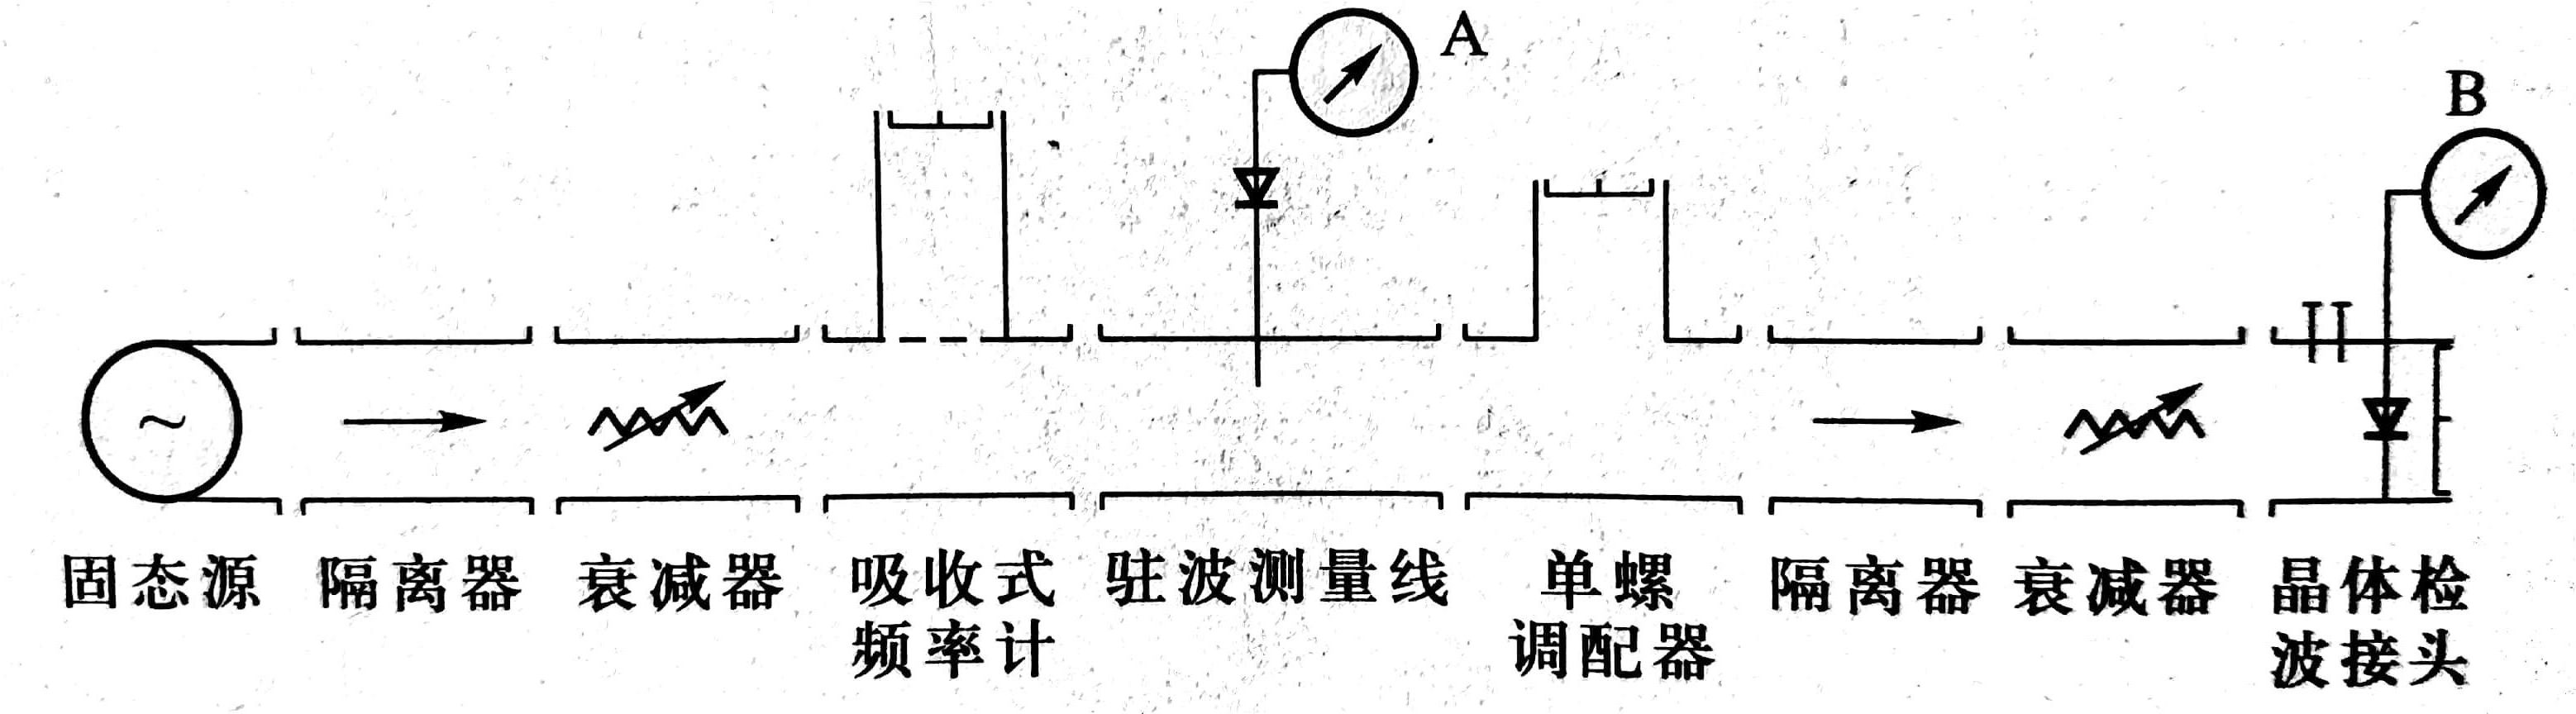
\includegraphics[width=120mm]{equip}
\caption{\label{fig:equip}%
实验装置图。它由永磁铁(约0.5T)、扫场线圈、探头、数字频率计、示波器、可调变压器、220V/6V小变压器及相移电路组成}
\end{figure}
如图\ref{fig:equip}所示。
\begin{enumerate}
\item 恒定磁场:由永久磁铁提供,大小约为0.5T。
\item 旋转射频磁场:由振荡线圈提供。被设置在$x$ 方向,振荡时沿此方向产生一个交变的线偏振场,$B_x = 2B_1\cos \omega t$, 这个线偏振场可以被分解为一个左旋分量和一个右旋分量,其中一个如果频率合适,可以被共振吸收;另一个由于与共振频率相差较大,对实验影响很小。
\item 边限振荡器接收信号:绕在样品上的线圈既作为振荡线圈产生射频场,也被用于接收信号。当共振发生时,样品吸收射频场能量,使得振荡线圈$Q$值减小,导致振荡器工作状态改变,表现在振荡波形的包络线发生变化,这就是共振信号。
\item 扫场:实验中采用扫场的方法探测核磁共振。固定射频场频率,让扫场$B'(t)$ 连续地变化,通过共振区域,产生可观测的吸收信号。实验中,可变的$B'(t)$ 由扫场线圈产生,它可以产生一个幅度在0 至0.001T 的正弦交变磁场,叠加在永磁铁产生的磁场上。$B'(t)=B' \sin \omega' t$,$\omega'=2\pi \times 50\mathrm{Hz}$为市电频率。所以$z$方向上的总磁场为
\begin{equation}
B=B_0+B'\sin \omega' t\label{eq:magnet}
\end{equation}

\end{enumerate}
\section{实验内容}
\subsection{定性观察加有顺磁剂的的水样品}\label{A}
观察掺有三氯化铁的水样品中质子的共振信号。将示波器设置为内扫描,速度置为2ms/格到5ms/格;增大扫场幅度至变压器数值为100,射频场频率为20.90MHz 附近时,观察到了质子的共振信号。找到质子共振信号后,改变下述条件观察共振信号的波形、幅度和位置分布的变化。
\subsubsection{增大射频场的频率$\nu$}\label{changefreq}
\begin{enumerate}
\item 位置分布变化:无信号$\to$每20ms的位置出现一个共振峰,渐渐分成两个$\to$20ms的峰位置不动,它们之间的峰位置从一个峰向另一个峰移动$\to$与另一个峰重合。

解释:共振峰位置由
\begin{equation}
\nu=|\frac{\gamma}{2\pi}|B=|\frac{\gamma}{2\pi}|(B_0+B'\sin \omega' t)\label{eq:reso}
\end{equation}
决定。当$\nu=|\frac{\gamma}{2\pi}|(B_0\pm B')$时,峰值位置(对应于扫场相位$\omega' t$)处于扫场信号的波谷或波峰处,两个峰就重合,相邻两峰的间距为扫场信号的周期20ms;当$|\frac{\gamma}{2\pi}|(B_0-B')<\nu<|\frac{\gamma}{2\pi}|(B_0+ B')$时,共振峰位置处在波谷和波峰之间,共振峰位置在一个周期内对应两个相位,当$\nu$由小到大增大时,峰值位置从波谷向波峰移动。

\item 波形变化:靠近波峰/波谷处尾波个数少,远离波峰/波谷处(靠近波节处)尾波个数多。

解释:式(\ref{eq:absorption})是基于稳态假设的,即通过共振区所需的时间要远比$T_1$和$T_2$长得多,这样才能观察到图(\ref{fig:absorption})的稳态信号。在波峰/波谷位置,外磁场变化速度较慢(正弦函数的导数较小),更接近稳态解,尾波相对较少;在波节位置,外磁场变化速度较快,瞬态现象(尾波)就更显著。

\item 幅度变化:越靠近波节位置信号强度越小,越靠近波峰/波谷处信号强度越大。

解释:靠近波节处扫场速度变快,使得信号偏离稳态,其结果将是得到的吸收信号强度减弱。相反,靠近波峰和波谷处信号更接近稳态解,信号强度也更强。
\end{enumerate}
\subsubsection{增大扫场幅度$B'$}
\begin{enumerate}
\item 位置分布变化:峰的位置向正弦扫场信号的零点移动,增大到一定程度后基本不变。

解释:仍由式(\ref{eq:reso})决定。$B'$增大后,等式成立对应的相位$\omega' t $向波节靠近。

\item 幅度变化:零扫场时观察几乎不到共振信号。出现共振信号后再加大扫场幅度时,扫场幅度一直减小。

解释:扫场幅度增大时,扫过共振对应的磁场大小附近时所用的时间相应的会更短,这就会使得得到的信号偏离稳态,系统还没有完全弛豫,其结果将是得到的吸收信号强度减弱。

\item 尾波变化:尾波拍频震动次数变多

解释:扫场幅度增大后,扫场弛豫时间$T_1$和$T_2$相较于加快了的扫场速度而言显得更长了,这使得尾波拍频数量变多。
\end{enumerate}
\subsubsection{改变电路盒的位置}
\begin{enumerate}
\item 位置分布变化:基本不变
\item 幅度变化:在两端不均匀处,信号峰幅度变小,宽度变大;在中间较均匀的区域幅度基本不变

解释:当电路盒位置移向磁场非均匀的地方时,由式(\ref{eq:effectiveT2})所示,有效横向弛豫时间$T_2^*$会变得更短,共振峰宽度将会相应地增加。另外,在两侧磁场不太均匀的地方,恒定磁场$B_0$的大小也有所减小,共振信号幅度将减小,共振峰将显得更加矮胖。

\item 尾波变化:不均匀处尾波震动次数变少。

解释:磁场强度越均匀的地方,由式(\ref{eq:effectiveT2})所示,有效横向弛豫时间$T_2^*$越长,能够观察到的尾波的拍频震动次数越多。

利用这一特点,我找到磁场最均匀处(尾波振动最多处)位于$1.0 \mathrm{cm}$刻度线处。
\end{enumerate}

\subsubsection{增大射频场幅度$B_1$}
共振信号的波形和位置分布基本不变,幅度先增大后减小。

解释:根据式(\ref{eq:absorption}),$v$随$B_1$确实是先增大后减小的。可以这样理解:增大射频场幅度$B_1$可以增加受激辐射和受激吸收的概率$P$,进而增
大共振吸收信号的幅度。但是当射频场幅度增大到一定程度时,
\begin{equation}
n_s =\frac{n_0}{1+2PT_1}\label{eq:saturate}
\end{equation}
上下能级粒子数差会变小,使得共振信号又开始减弱。

记下并保持共振信号幅度最大时的“幅度调节”旋钮指针位置:5.50。
\subsection{在共振条件下校准磁场}\label{B}
已知$25\degree\mathrm{C}$球形水样品中质子的回旋频率
\begin{equation}
\left(\frac{\gamma}{2\pi}\right)_H=42.576 388 8\pm0.000 001 8 \mathrm{MHz/T}
\end{equation}
(不确定度$\sim 10^{-8}$,可忽略)作为标准值校准永磁体的磁场。

保持\ref{A}中的电路盒位置和射频场幅度。由\ref{eq:magnet},总磁场由$B_0$和$B' \sin \omega' t$两部分组成。因此当共振信号均匀排列且间隔为10 ms时对应于共振发生在扫场过零时刻,这时频率计的读数才是与$B_0$对应的共振频率。

由于只要观察到共振信号,$B_0$的测量误差不会超过扫场的幅度$B'$,因此,为了减少$B_0$的测量误差,在找到共振信号后应逐渐减小扫场的幅度并把$B'$减小到尽可能小。在减小$B'$的过程中同时调节频率,使共振信号保持均匀分布而且间隔10 ms 排列。当$B'$已经足够小时,读出这时的频率作为与$B_0$的共振频率:
\begin{equation}
\nu_H=20.89068 \mathrm{MHz}
\end{equation}
则
\begin{equation}
B_0=\nu_H/\left(\frac{\gamma}{2\pi}\right)_H=0.490664 \mathrm{T}
\end{equation}

为了定量的估计$B_0$的误差,在扫场幅度足够小的前提下,保持扫场幅度不变,调节频率,使共振先后发生在扫场的波峰(此时$B=B_0+B'$,$\nu_H'>\nu_H$)和波谷(此时$B=B_0-B'$,$\nu_H''<\nu_H$)。在这个过程中,在示波器上观察到原先间隔为10 ms的均匀排列的共振信号中,有两个相邻的峰逐渐靠拢合并成一个峰,从而共振峰数目减少一半,相邻的共振信号间隔变为20 ms,记下共振发生在扫场波峰与波谷的共振频率$\nu_H'$和$\nu_H''$:
\begin{equation}
\nu_H'=20.89936\mathrm{MHz},\ \nu_H''=20.88191\mathrm{MHz}
\end{equation}
则可以估测此时的扫场幅度$B'$:
\begin{equation}
B'=\frac{(\nu_H'-\nu_H'')/2}{(\gamma/2\pi)_H}=2.05\times 10^{-4} \mathrm{T}
\end{equation}
粗略的估计可取$B'$的$1/10$作为$\Delta B_0$的估计误差:
\begin{equation}
\Delta B_0=\frac{B'}{10}=2\times 10 ^{-5} \mathrm{T}
\end{equation}
此时的相对不确定度$\frac{\Delta B_0}{B_0}=4\times 10 ^{-5}$,
\begin{equation}
B_0\pm \Delta B_0 =(0.49066 \pm 0.00002 ) \mathrm{T}
\end{equation}

\subsection{观察聚四氟乙烯中$\F$核的共振信号,测量其$g$因子}
首先找到共振信号。与水的共振信号相比,聚四氟乙烯的信号较弱,这时由于;共振峰几乎观察不到尾波,这是因为固体的横向弛豫时间$T_2$比液体短得多,远远小于扫场的周期,从而符合稳态近似。

完全类似\ref{B}中的操作,在扫场幅度足够小的条件下,调节频率使得共振信号均匀分布,间隔10 ms,这时的频率为$\F$核与$B_0$对应的共振频率
\begin{equation}
\nu _F =19.65386 \mathrm{MHz}
\end{equation}
则用已经校准的磁场$B_0$和常量$\mu_N / h=(7.62259396 \pm 0.00000031 \mathrm{MHz/T})$(同样,不确定度$\sim 10^{-8}$,可忽略)可以求出$\F$核的$g$因子
\begin{equation}
g=\frac{\nu_F / B_0}{\mu_N / h}=\frac{19.65386/0.49066}{7.622594}=5.2549
\end{equation}
与\ref{B}中类似,通过波峰处对应的频率$\nu_F'$和波谷处对应的频率$\nu_F''$
\begin{equation}
\nu_F'=19.66812\mathrm{MHz},\ \nu_F''=19.64041\mathrm{MHz}
\end{equation}
与\ref{B}中类似地,估计$\nu_F$的相对不确定度:
\begin{equation}
\frac{\Delta \nu_F}{\nu_F}=\frac{(\nu_F'-\nu_F'')/20}{\nu_F}\approx 7\times 10^{-5}
\end{equation}
从而$g$的相对不确定度
\begin{equation}
\frac{\Delta g}{g}=\sqrt{\left(\frac{\Delta B_0}{B_0}\right)^2+\left(\frac{\Delta \nu_F}{\nu_F}\right)^2}=\sqrt{4^2+7^2}\times 10 ^{-5}\approx8\times 10 ^{-5}
\end{equation}
则$\F$核$g$因子的测量结果为
\begin{equation}
g\pm\Delta g =5.2549\pm0.0004
\end{equation}
\subsection{比较“纯水”样品与掺有三氯化铁的水样品中质子的共振信号}
与加入顺磁剂的水的共振信号相比,纯水的共振信号幅度要弱很多,由于系统存在一定的噪声,这导致纯水的信号较不清晰,无法分辨尾波等结构。这主要是由于纯水中没有掺杂顺磁离子,磁矩的弛豫时间$T_1$较长,使得式(\ref{eq:saturate})中的饱和因子$z$很小,上下能级的粒子数差$n_s$就很小,因而信号表现得很弱。
\subsection{估测聚四氟乙烯样品中$\F$核的横向弛豫时间$T_2$}
将示波器改用X-Y输入方法,X端输入扫场信号,Y端输入“检波输出”信号。调节频率在$\nu_F$附近并适当增大扫场幅度,从示波器上观察到重叠而又相互错开的两个共振峰。利用示波器上的网格估测其中一个共振峰的半宽
$$\Delta B=0.115 \mathrm{V}$$
另外,测出扫场变化范围$2B'$:
$$2B'=1.780 \mathrm{V}$$
从而得到比值$k=\Delta B /2B'=0.0646$,以此来对示波器的X轴进行定标。然后固定扫场的幅度不变,仍改回单通道,用于\ref{A}中完全类似的方法,测得共振发生在扫场的波峰与波谷时的共振频率:
\begin{equation}
\nu_F'=19.7017\mathrm{MHz}, \ \nu_F''=19.6125\mathrm{MHz}
\end{equation}
$\Delta \omega =\Delta B \gamma= k \cdot 2B' \gamma =k \cdot 2\pi (\nu_F'-\nu_F'')$。从而估测横向弛豫时间出$T_2$:
\begin{equation}
T_2=\frac{2}{\Delta \omega}=\frac{1}{\pi k (\nu_F'-\nu _F'')}=5.52\times 10 ^{-5}\mathrm{s}
\end{equation}
\section{结论}
本实验利用扫场的测量方法观测了掺有顺磁剂的水、聚四氟乙烯、纯水三种样品的核磁共振信号,定性地研究了信号在各种参量影响下会发生的变化,验证了核磁共振宏观理论的
合理性。利用水样品中质子的核磁共振信号校准了恒定磁场的大小$B_0 =(0.49066 \pm 0.00002 ) \mathrm{T}$。利用校准后的磁场,确定了聚四氟乙烯中$\F$核的$g$因子为$5.2549\pm0.0004$,估测了横向弛豫时间为$5.52\times 10 ^{-5}\mathrm{s}$。通过比对纯水与水的样品的核磁共振信号,验证了弛豫时间对信号强度、波形的影响。

\section{致谢}
感谢黄斐增老师的耐心指导以及在原理部分的深入讲解。

\appendix
\section{思考题}
\subsection{实验过程思考题}
\subsubsection{当示波器采用内部线性扫描时,一开始若找不到共振信号,有哪几种可能的原因?找到信号后,改变射频场频率时,共振信号在荧光屏上的分布如何变化?在什么情况下读取的频率才是与$B_0$对应的共振频率?}
若一开始找不到共振信号,可能是射频场幅度$B_1$太大或太小,射频场频率$\omega$与共振频率$\omega_0$相差太远,或者扫场幅度$B'$太小。

其余所有思考题的回答都已在正文中给出。

\end{document}
